\documentclass[11pt]{article}
\usepackage{graphicx}
\usepackage{caption}
\usepackage{hyperref}
\usepackage{amsmath}
\usepackage{amssymb}
\usepackage[margin=1.5in]{geometry}

\begin{document}
% Critique the most important figure from a seminal paper in your field. Provide the original figure/caption. In your own words, what story is this figure trying to convey? What does it do well? What could have been done better? What elements didn't need to be present to still convey the same story?
I chose the figure from the Planck 2013 data release showing the temperature power spectrum of the cosmic microwave background. This is my favourite figure because the standard $\Lambda$CDM model of cosmology fits so well and I think it's really cool that so few parameters can predict the power spectrum so well!

The figure summarizes all of the temperature data taken by Planck neatly, and shows how well our standard cosmological model fits the data. It's very successful at collapsing an enormous amount of data into one figure to compare with theory. Often one of the hardest parts of making these kinds of plots is to make sure you are using all of the data and information you have, and still can compare to theory. I think this plot collapses that problem neatly, and the error bars and $\ell$ bins make sense and are aesthetically pleasing.

I think maybe something the figure isn't as successful on is the slightly confusing scale changes. The plot switches from log to linear on the $x$ axis at $\ell = 50$. This is definitely necessary to see all of the data in the low $\ell$ range, but it does make it slightly harder to understand at a glance. I do think the dotted line helps a lot with that. The most confusing scale change is the $y$ axis in the residual plots, where the vertical scale changes at $\ell = 50$. I do think this helps to show the residuals for higher $\ell$ better, and the confusion is lessened by having this explicitly written in the last sentence of the caption.

I think the part of the plot I understand the least is the green lines on the bottom plot, and I'm not sure they are necessary. It seems that the residuals would look much cleaner without the lines here. I also think the colour is somewhat challenging visually.

On an aesthetics note, I really think the plot could use a different font and different plot labelling. The font just doesn't look great and doesn't match the body of the paper, and additionally looks pretty dated. The math formatting is also not very appealing, and does not look like the nice LaTeX typesetting we are all familiar with. It feels like maybe the labels could have been added in after the fact to look nicer and more modern. I think that overall the font choice is my least favourite part of this plot.

\begin{figure}[h]
\begin{center}
	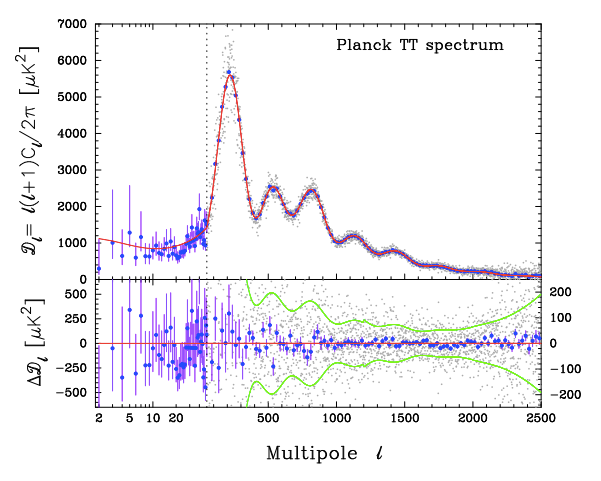
\includegraphics[width=\textwidth]{hw_2_data/planck_plot_moreinfo.png}
\caption{\small This figure was taken from [1]. The caption there is:
Planck foreground-subtracted temperature power spectrum (with foreground and other nuisance parameters fixed to their best-fit values for the base $\Lambda$CDM model). The power spectrum at low multipoles $\ell$ = 2-49, plotted on a logarithmic multipole scale) is determined by the Commander algorithm applied to the Planck maps in the frequency range 30-353 GHz over 91\% of the sky. This is used to construct a low-multipole temperature likelihood using a Blackwell-Rao estimator, as described in Planck Collaboration XV (2014). The asymmetric error bars show 68\% confidence limits and include the contribution from uncertainties in foreground subtraction. At multipoles 50 $< \ell <$  2500 (plotted on a linear multipole scale) we show the best-fit The CMB spectrum computed from the CamSpec likelihood (see Planck Collaboration XV 2014) after removal of unresolved foreground components. This spectrum is averaged over the frequency range 100-217 GHz using frequency-dependent diffuse sky cuts (retaining 58\% of the sky at 100 GHz and 37\% of the sky at 143 and 217 GHz) and is sample-variance limited to $\ell$ = 1600. The light grey points show the power spectrum multipole-by-multipole. The blue points show averages in bands of width $\Delta \ell \approx 31$ together with 1$\sigma$ errors  computed from the diagonal components of the band-averaged covariance matrix (which includes contributions from beam and foreground uncertainties). The red line shows the temperature spectrum for the best-fit base $\Lambda$CDM cosmology. The lower panel shows the power spectrum residuals with respect to this theoretical model. The green lines show the $\pm 1\sigma$ errors on the individual power spectrum estimates at high multipoles computed from the CamSpec covariance matrix. Note the change in vertical scale in the lower panel at $\ell$ = 50.}
\label{fig.1}
\end{center}
\end{figure}

\section*{Reference}
[1]  Planck 2013 results. XVI. Cosmological parameters - Planck Collaboration (Ade, P.A.R. et al.) Astron.Astrophys. 571 (2014) A16 arXiv:1303.5076 [astro-ph.CO] 

\end{document}